\chapter{Hydrogen bond dynamics and instantaneous interfaces}
\section{Relations between HB lifetime distributions}\label{relation_hbd}
%Why is the lifetime of H-bonds worth paying attention to?
%The HB lifetime is a significant feature of H-bonds in liquids. 
The peculiar properties of water are a direct consequence of water's HB lifetime distribution\cite{Lee2007,Sciortino1989,Sciortino1990prl}.
For example, understanding of HB dynamics is essential when investigating proton transfer reactions in protein environments\cite{Ishikita2013}.  
The statistical properties of lifetime of H-bonds can be described by a variety of distribution functions{\cite{Rapaport1983, Tanaka1983, Geiger1984,Naberukhin2009}.
Below we discuss the three probability distribution functions of HB lifetime, so that we can study the dynamic characteristics of H-bonds in liquids and interfaces.

\paragraph{Probability distribution of HB lifetimes in a configuration}\label{P_tc}
Suppose that there are $n_\text{tot}$ H-bonds in a system at time $t$, and we can distinguish a part of H-bonds from these H-bonds. 
The lifetime of this part of H-bonds is in a certain range $[\tau, \tau + d\tau]$. We can assume that their number of those bonds is $n_\tau$. 
One can easily find that $n_\text{tot}>n_\tau$. If we observe this part of H-bonds in the next time period $[t, t+\tau]$, 
then they will be broken once during $[t, t+\tau]$. 
That is to say, within $[t,t+\tau]$, we will detect the breaking of all H-bonds with lifetime $\tau$ (Fig. \ref{fig:P_tc}).  
Therefore, in a short period of time $d\tau$, the probability of detecting these H-bonds is $(1/\tau)d\tau$.
Since the probability for the HB to have the lifetime $\in [\tau,\tau+d\tau]$ is $P_\text{t}(\tau)$. 
Therefore, the relation between $P_\text{a}(t)$ and $P_\text{t}(t)$ is
\begin{eqnarray}
P_\text{a}(t) = \int_t^\infty P_\text{t}(\tau)\frac{d\tau}{\tau},
\label{eq:Pt_and_P}
\end{eqnarray}
i.e., the probability of the HB breaking for the first time in the time $t$ after detection at the initial moment depends on 
the number of those H-bonds whose lifetime exceeds the given time $t$\cite{Voloshin2009}.
\begin{figure}
\centering
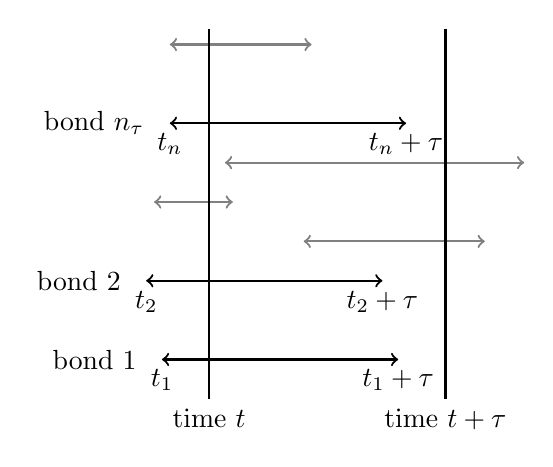
\begin{tikzpicture}[help lines/.style={thin,draw=black!50}]
%%\draw[help lines] (0,0) grid (4,4);
\draw [<->, thick] (0.4,0) node [anchor = north] {$t_1$} -- (3.4,0) node [anchor = north] {$t_1 + \tau$};
\draw (0.2,0) node [anchor = east] {bond $1$};
\draw [<->, thick] (0.2,1) node [anchor = north] {$t_2$} -- (3.2,1) node [anchor = north] {$t_2 + \tau$};
\draw (0,1) node [anchor = east] {bond $2$};
\draw [<->, thick] (0.5,3) node [anchor = north] {$t_n $} -- (3.5,3) node [anchor = north] {$t_n + \tau$};
\draw (0.3,3) node [anchor = east] {bond $n_{\tau}$};
\draw [gray,<->, thick] (1.2,2.5) -- (5.0,2.5);
\draw [gray,<->, thick] (0.3,2) -- (1.3,2);
\draw [gray,<->, thick] (2.2,1.5) -- (4.5,1.5);
\draw [gray,<->, thick] (0.5,4) -- (2.3,4) ;
\draw [thick] (1.0,4.2) -- (1.0,-0.5) node [anchor = north] {time $t$};
\draw [thick] (4.0,4.2) -- (4.0,-0.5) node [anchor = north] {time $t+\tau$};
\end{tikzpicture}
  \caption{\label{fig:P_tc} The H-bonds with lifetime $\tau$ in a certain configuration. 
At time $t$, we assume that there are totally $n_\text{tot}$ H-bonds can be detected, and $n_{\tau}$ H-bonds are of lifetime $\tau$, therefore,  the fraction of H-bonds that 
have the lifetime $\tau$ in the configuration at time $t$ is $P_\text{tc}(\tau) =  n_{\tau} /n_\text{tot}$.
Let $\tau$ take all the values in the interval $[0,\infty]$, we can get the HB lifetime distribution $P_\text{tc}(t)$.
}
\end{figure}

\paragraph{HB lifetime distributions}\label{diff_distr}
From the probability $P_\text{tc}(t)$ of the total HB lifetime in a configuration, and the probability $P_\text{a}$ of 
the first HB breaking in time $t$ after it have been detected at the moment $t$, one can introduce the average time 
$\langle \tau_\text{tc}\rangle$ and $\langle \tau_\text{a}\rangle$ :
\begin{equation}
\langle \tau_\text{tc}\rangle = \int_0^\infty t P_\text{tc}(t) dt,
\label{eq:tau_tc}
\end{equation}
\begin{equation}
\langle \tau_\text{a}\rangle = \int_0^\infty t P_\text{a}(t) dt. 
\label{eq:tau_a}
\end{equation}
Since $P_{\mathrm{a}}(t)=\int_{t}^{\infty} P_{\mathrm{tc}}(\tau) \frac{d \tau}{\tau}$, i.e., 
\begin{equation}
P_\text{tc}(t) = -t\frac{dP_\text{a}(t)}{dt}, \nonumber
\label{eq:relation_Ptc--Pa}
\end{equation}
integrating by parts, we obtain
\begin{eqnarray}
&&\langle \tau_\text{tc}\rangle = -\int_0^\infty t^2 \frac{dP_{\mathrm{a}}(t)}{dt}dt \nonumber \\
%
&&= -\int_0^\infty t^2 dP_\text{a}(t) \nonumber\\
&&= 2\langle \tau_\text{a}\rangle,\nonumber
\end{eqnarray}
in which we used $\int_0^\infty d(t^2 P_\text{a})=0$.

We denote the probability of the total HB lifetime along a trajectory as $P_{\mathrm{tt}}(t)$,
then the average HB lifetime over the trajectory is
\begin{eqnarray}
\left\langle\tau_{\mathrm{tt}}\right\rangle=\int_{0}^{\infty} t P_{\mathrm{tt}}(t) d t.
\label{eq:relation_tau_tt}
\end{eqnarray}
Because $\int_{0}^{\infty} P_{\mathrm{tc}}(t) d t=\frac{1}{\langle \tau_\text{tt}\rangle} \int_{0}^{\infty} t P_{\mathrm{tt}}(t) d t = 1$, 
we get 
\begin{eqnarray}
P_{\mathrm{tt}}(t)=\left\langle \tau_{\mathrm{tt}}\right\rangle P_{\mathrm{tc}}(t) / t.
\label{eq:relation_P_tt--P_tc}
\end{eqnarray}
The difference between the distribution functions, $P_{\mathrm{tt}}(t)$ and $P_{\mathrm{tc}}(t)$, can be described as follows.
$P_{\mathrm{tt}}(t)$ represents the percentage of pairs of molecules that had a continuous H-bonds during time $t$, 
while $P_{\mathrm{tc}}(t)$ the percentage of the number of H-bonds with a given lifetime $t$ 
to the number of all H-bonds in any configuration\cite{Voloshin2009}.

Since $P_{\mathrm{a}}(t)=\int_{t}^{\infty} P_{\mathrm{tc}}(\tau) \frac{d \tau}{\tau}$,
we can obtain
\begin{eqnarray}
&& P_{\mathrm{a}}(t)=\int_t^\infty \frac{P_\text{tt}}{\langle\tau_\text{tt}\rangle} \frac{\tau}{\tau} d\tau \nonumber \\
&& =  \int_t^\infty \frac{P_\text{tt}}{\langle\tau_\text{tt}\rangle}d\tau. \nonumber
\label{eq:P_a}
\end{eqnarray}
Let $t=0$, we have 
\begin{eqnarray}
P_{\mathrm{a}}(0)=1 /\left\langle t_{\mathrm{tt}}\right\rangle = 1 /\left\langle t_{\mathrm{HB}}\right\rangle.
\label{eq:P_a0}
\end{eqnarray}

From Eq. \ref{eq:tau_tc} and the relation between \SHB and $P_{\mathrm{a}}(t)$
\begin{eqnarray}
s(t)=\int_{t}^{\infty} P_{\mathrm{a}}(\tau) d \tau,
\label{eq:P_a}
\end{eqnarray}
we obtain
%
\begin{eqnarray}
&&\int_{0}^{\infty} \int_{t}^{\infty} P_\text{a}(t) d \tau d t = \int_{0}^{\infty} \int_{0}^{\tau} P_\text{a}(\tau) d t d \tau \nonumber \\
&& = \int_{0}^{\infty} \tau P_\text{a}(\tau) d \tau \nonumber \\
&& = \langle \tau_{\mathrm{a}} \rangle, \nonumber
\end{eqnarray}
i.e., 
\begin{eqnarray}
\int_{0}^{\infty} s(t) d t = \langle \tau_{\mathrm{a}} \rangle.
\label{eq:int_Ca}
\end{eqnarray}
\paragraph{Calculation of HB lifetime distributions}
In this paragraph, we describe the method to calculate the above lifetime distributions $P_\text{tc}(\tau)$, $P_\text{a}(\tau)$, and $P_\text{tt}(\tau)$.

First, we describe the method of calculating $P_\text{tc}(\tau)$.
Theoretically speaking, in order to calculate $P_\text{tc}(\tau)$, our detection time $t$ must meet the following conditions: 
$t-t_0 > \tau_\text{hb}^{\max}$, where $t_0$ is the initial time and $\tau_\text{hb}^{\max}$ is the maximum lifetime value of the H-bonds in the system. 
However, the value of $\tau_\text{hb}$ cannot be known in advance. 
In order to reduce the error, the method we can adopt is to set an empirical value as large as possible for
 $\tau_\text{hb}^{\max}$ if conditions permit. Since the value of $\tau_\text{hb}^{\max}$ is limited, in principle the lifetime value of the HB 
can always be greater than $\tau_\text{hb}^{\max}$. 
Therefore, the average value of the HB lifetime distribution 
calculated in this approximate way will move to a shorter lifetime than the average value of the true HB lifetime distribution:
\begin{eqnarray}
\int_{0}^{\infty} \tau P_{\mathrm{tc}}^{\mathrm{approx}}(\tau) d \tau < \left\langle\tau_{\mathrm{tc}}\right\rangle.
\label{eq:upper_bound_1_for_tau_tc}
\end{eqnarray} 

Among H-bonds detected at time $t$, if there are H-bonds that have existed at the beginning $t_0$ and 
remain in existence until time $t$, then we can approximately express the lifetime of these H-bonds as $\delta t^{(j)}=t^{(j)} -t_0$, 
where $j=1,\cdots, m$ is the labels of the $m$ H-bonds and $t^{(j)}$ is the moment when the $j$-th HB is broken. 
If we use $\tau^{(j)},j=1,\cdots,m$ to represent the true lifetimes of these $m$ H-bonds,
then we can find that $\tau^{(j)}-\delta t^{(j)} >0 $.
Since we cannot judge the true lifetime of these H-bonds, we can use $\delta t^{(j)}$ to approximate 
the lifetime of these $m$ H-bonds, that is
\begin{eqnarray}
\tau^{(j)} = \delta t^{(j)}, j=1,\cdots,m.
\end{eqnarray}
For those H-bonds that did not exist at the beginning, the method of calculating their lifetime is straightforward, 
the lifetime $\tau^{(j)}$ is equal to the time $t^{(j)}$ when the HB is broken minus the time $t^{{(j)}}_0$ of its formation:
\begin{eqnarray}
\tau^{(j)} = t^{(j)} - t^{(j)}_0,
\end{eqnarray} 
where the superscript $j = 1, \cdots, m'$, identifies $m'$ H-bonds 
detected at time $t$, and
formed after $t_0$ and broken at $t^{(j)}$.

Specifically, for DFTMD results, we approximate $P_\text{tc}$ as follows: 
We select evenly distributed $n$ time points $t=t_1,...,t_n$, from the trajectory obtained by the simulation, 
and count the HB lifetime at each time point $t_i$.
The distribution $P_\text{tc}(\tau)$ 
can be obtained by the average of the lifetime distribution detected at a certain time $t_i$, $i=1,\cdots, n$, 
where $t_i-t_{i-1} = \tau_\text{hb}^{\max}$. 

From the perspective of simulation data, we have another way to obtain $P_\text{tc}(\tau)$: 
Count the lifetimes of H-bonds that are formed after the initial time $t_0$ and are broken before the end time $t_\text{f}$.
%Although the distribution obtained in this method cannot be verified experimentally, it is the true distribution of HB bonds in simulated systems. 

\section{HB population operator}\label{hbpo}
\paragraph{Calculation of the reactive flux}\label{calc_rf}
For dynamical variables $x_i(t)$ and $x_k(t)$, their correlation functions have the following relationship\cite{Landau1980}:
\begin{equation}
\langle x_i(t') x_k(t)\rangle = -\langle x_i(t) x_k(t')\rangle.
\label{eq:correlation_relation}
\end{equation}
Let $x_i = h$, $x_k = \dot h$,
then, we obtain
\begin{equation}
\langle h(0) \dot{h}(t)\rangle=-\langle\dot{h}(0) h(t)\rangle. 
\label{eq:h_correl_relation}
\end{equation}
From the definition of the reactive flux $k(t) = -dc/dt$, we obtain 
\begin{equation}
k(t)=-\langle h(0) \dot{h}(t)\rangle /\langle h\rangle. 
\label{eq:rf1}
\end{equation}
Then from Eq. \ref{eq:h_correl_relation},
we get 
\begin{equation}
k(t) =  \langle \dot{h}(0)h(t)\rangle /\langle h\rangle. \nonumber
\label{eq:rf2}
\end{equation}
Since $\langle\dot{h}(0)\rangle=0$, $k(t)$ can be calculated by
\begin{equation}
k(t) = - \langle \dot{h}(0)[1-h(t)]\rangle /\langle h\rangle.
\label{eq:rf3}
\end{equation}


\paragraph{Relaxation time of H-bonds in bulk water}\label{rate_const_and_tau_R_128w}
% 
For the dynamic trajectory of such a system, we also calculated the self-correlation function $c(t)$ of the HB population operator, 
and the functions $k(t)$ and $n(t)$ derived from it. 
Tables \ref{tab:k_k_prime_128w_1} and \ref{tab:k_k_prime_128w_2} show the rate constants $k$ and $k'$, and 
the relaxation time $\tau_\text{HB}$ obtained by the least squares fit method. 
%It can be seen from the tables that the accuracy of the calculation of $k$, $k'$ are accurate to at least two decimal places.

%
\begin{table}[H] %[htbp]
\centering
\caption{\label{tab:k_k_prime_128w_1} 
    The $k$ and $k'$ for bulk water. We carried on the short time region 0.2 ps $< t <$ 2 ps. 
The unit for $k$ ($k'$) is ps$^{-1}$, and that for $\tau_{\text{HB}}$ ($=1/k$) is ps. The $h(t)$ is bond-based.} 
\begin{tabular}{cccc}
 Criterion & $k$  (bulk) & $k'$ (bulk) & $\tau_{\text{HB}}$ (bulk) \\
\hline
  %ADH & 0.335 & 0.937 & 2.988  \\
  %ADH(from $k_{in}$) & 0.299  & 1.029 & 3.347   \\
  %AHD & 0.322 & 1.01 & 3.101 \\ 
  %AHD(from $k_{in}$) & 0.288 & 1.121 & 3.468 \\ 
  ADH & 0.299  & 1.029 & 3.347   \\
  AHD & 0.288 & 1.121 & 3.468 \\ 
\end{tabular}
\end{table}
%
\begin{table}[H]%[htbp]
\centering
\caption{\label{tab:k_k_prime_128w_2} 
    The $k$ and $k'$ for bulk water. We carried on the long time region 2 ps $< t <$ 12 ps. 
The unit for $k$ ($k'$) is ps$^{-1}$, and that for $\tau_{\text{HB}}$ ($=1/k$) is ps. The $h(t)$ is bond-based.} 
\begin{tabular}{cccc}
 Criterion & $k$  (bulk) & $k'$ (bulk) & $\tau_{\text{HB}}$ (bulk) \\
\hline
  %ADH & 0.103 & 0.024 & 9.690 \\
  %ADH(from $k_{in}$) & 0.103  & 0.028 & 9.728 \\
  %AHD & 0.104 & 0.034 & 9.656  \\
  %AHD(from $k_{in}$) & 0.103  & 0.040 & 9.702  \\
  ADH & 0.103  & 0.028 & 9.728 \\
  AHD & 0.103  & 0.040 & 9.702  \\
\end{tabular}
\end{table}

%\paragraph{Different definitions of the $h(t)$}\label{DEF_POPULATION_OPERATOR}
%Here we discuss the definition of another possible hydrogen bond population operator $\tilde{h}(t)$ besides $h(t)$ introduced in the text.
%When a pair of water molecules $a$ and $b$ are H-bonded, 
%the oxygen atom in each water molecule can act both as a donor and an acceptor. 
%In particular, a pair of water molecules can form 4 different forms of H-bonds. 
%In other words, if the role of H atoms between the pair of water molecules changes, but they still form H-bonds, 
%we think that an old H-bond is broken and a new H-bond is formed.

%The correlation functions \CHB of water molecules in bulk water is shown in Fig. \ref{fig:bk_water_c_two_population_operators_with_ADH}.
%It shows that there are big differences in the correlation functions of the two definitions $h(t)$ and $\tilde{h}(t)$,
%because hydrogen exchange is considered in the O--H pair-based HB population $\tilde{h}(t)$, but not in the W--W pair-based HB population $h(t)$.
% bk_water_c_two_population_operators_with_ADH.eps
% /home/gang/Github/water_pair_HB_dynamics/plot/plot_c/bk_water_c_two_population_operators_with_ADH.eps
% old version: 128w_bk--water-pair-based_and_bond-based_c.eps
%\begin{figure} [htbp]
%\centering
%	\includegraphics [width=0.36\textwidth] {./diagrams/bk_water_c_two_population_operators_with_ADH}
%\setlength{\abovecaptionskip}{0pt}
%	\caption{\label{fig:bk_water_c_two_population_operators_with_ADH} The correlation functions \CHB of water molecules in bulk water (ADH criterion). 
%        Here HB population is based on two different definitions, one is based on a pair of water molecules (solid line),\cite{Khaliullin2013} 
%and the other is based on O--H pairs between water molecules (dashed line).}
%\end{figure} 

%\section{Fitting $C_2(t)$ with a single exponential function}\label{single_exp}
%We assume that the anisotropy decay $C_2(t)$ is a single exponential given by 
%\begin{equation}
%C_2(t) = A e^{-\kappa t},
%\label{eq:tcf2}
%\end{equation}
%where $\kappa$ is a relaxation rate constant of the anisotropy decay. For each value of $\kappa$, we denote the relaxation period as $1/\kappa$.
%The $C_2(t)$ for water molecules in different environments in LiI solution at 330 K is shown in
%Fig.\thinspace\ref{fig:2LiI-124w_c2_fit_5_single-exp}.
%\begin{figure} [htbp]
%\centering
%	\includegraphics [width=0.60\textwidth] {./diagrams/2LiI-124w_c2_fit_5_single-exp}
%\setlength{\abovecaptionskip}{0pt}
%	\caption{\label{fig:2LiI-124w_c2_fit_5_single-exp} The anisotropy decay of OH bonds in water molecules at the interface of LiI solutions.}
%\end{figure} 
%It is evident, from the figure, that $C_2(t)$ for water molecules neither in the bulk or at interface of the LiI solution can \emph{not} be described as a single exponential dynamics.  Besides, we also have fitted the $C_2(t)$ for water molecules in NaI solution and the result is the same as above. The fitting parameters for LiI and NaI solution are presented in table \ref{tab:c2_single-exp-fitting_LiI} and \ref{tab:c2_single-exp-fitting_NaI}, respectively.
%%-- 
%\begin{table}
%\centering
%\caption{\label{tab:c2_single-exp-fitting_LiI}%
%	The single-exponentially fitted parameters---the amplitude $A$, the decay rate $\kappa$, the relaxation period $1/\kappa$, of anisotropy decay for water molecules 
%  at the interface of 0.9 M LiI solutions, at 330 K.} 
%\begin{tabular}{lccc}
%	water molecules &  $A$ & $\kappa$ (THz) & $1/\kappa$ (ps)  \\
%\hline
%	I$^-$-shell  & 0.83  & 0.26  & 3.85  \\
%	Li$^+$-shell & 0.89  & 0.07  & 14.29 \\
%	bulk & 0.86 & 0.12 & 8.33 \\
%	surface & 0.75 & 0.29 & 3.45 \\
%\end{tabular}
%\end{table}
%%-- 
%\begin{table}[H]
%\centering
%\caption{\label{tab:c2_single-exp-fitting_NaI}%
%	The single-exponentially fitted parameters---the amplitude $A$, the decay rate $\kappa$, the relaxation period $1/\kappa$, of anisotropy decay for water molecules 
%	at the interface of 0.9 M NaI solutions, at 330 K.} 
%\begin{tabular}{lccc}
%	water molecules &  $A$ & $\kappa$ (THz) & $1/\kappa$ (ps)  \\
%\hline
%	I$^-$-shell  & 0.86  & 0.14  & 7.14 \\
%	Na$^+$-shell & 0.79 & 0.07  & 14.29 \\
%	bulk & 0.83 & 0.06  & 16.67 \\
%	surface & 0.78 & 0.12 & 8.34 \\
%\end{tabular}
%\end{table}

%\section{Reorientation dynamics of water molecules at solution/vapor interfaces}\label{C2_DOUBLE_FIT}
%\paragraph{Double exponential fit}
%In general, the rotational motion of water molecules are not simply characterized by a well-defined rate constant. 
%Similar non-single-exponential kinetics is also obtained in HB dynamics 
%in liquid water\cite{AL96,Dirama2005} and in the time variation of the average frequency shifts of the 
%remaining modes after excitation in hole burning technique\cite{Rey2002,Moller2004}.
%We can understand the non-single-exponential kinetics of rotational 
%anisotropy decay by fitting the rotational anisotropy decay by a 
%biexponential function.

%To obtain the effects of diffusion and HB decay of water molecules
%in solutions respectively, we assume that 
%the correlation function $C_2(t)$ has the form\cite{TanHS2005}
%\begin{equation}
%C_2(t)=A_1e^{-t/\tau_{2,1}} +A_2e^{-t/\tau_{2,2}},
%\label{eq:tcf3}
%\end{equation}
%where $A_i$ are amplitudes and $1/\tau_{2,i}$ ($i=1, 2$) are decay rates of $C_2(t)$,
%and the $\tau_{2,i}$ represent the relaxation times of the $C_2(t)$. 
%%(DONE: Here I should comment on which is the physical meaning of a double exponential.)
%Here, we assume that the orientation relaxation $C_2(t)$ is composed of two independent relaxation processes 
%with different time scales, and each process can be described by an exponential decay function, respectively.
%For alkali-iodine solutions (LiI and NaI), the $A_i$ and $\tau_{2,i}$ of the biexponentials fits for functions 
%$C_2(t)$ are shown in Table ~\ref{tab:table8}.
%%As an example, for the interface of LiI solution, we made a comparison between $C_2(t)$ 
%%and the function fitted according to Eq.\thinspace\ref{eq:tcf3},
%%as shown in Fig.\thinspace\ref{fig:2LiI-124w_c2_fit_5ps_biexp}. 
%We found that Eq. \ref{eq:tcf3}, the biexponential kinetics is sufficiently accurate to 
%describe the characteristics of anisotropy decay.                        

%Then we considered the effect of ion species in solution/vapor interfaces on the anisotropy decay of water molecules.
%%(DONE: Here is on the surface or not? interfaces.).
%For both LiI and NaI solutions, there are two decay processes 
%(Table \ref{tab:table8})
%--- amplitude $\sim 1$,
%decay time $\tau_{2,2}\sim$ 10.0 ps, and for the other describe the initial fast decay 
%of the anisotropy, with amplitude $\sim 0.1$, decay time $\tau_{2,1}\sim$ 0.1--1.0 ps, 
%due to the inertial--librational motion preceding the orientational diffusion.
%%The one describe the initial fast decay of the anisotropy, 
%%with amplitude $\sim$ 0.1, decay constant $\sim$ (1--10) THz,
%%results from the inertial-librational motion preceding the orientational diffusion.
%%


%%{Fitting by a biexponential}
%\begin{table}[H]  % or [!htbp]
%\centering
%\caption{\label{tab:table8}
%The fitted parameters of anisotropy decay of water molecules at the LiI (NaI, KI) solution/vapor interface 
%according to Eq. \ref{eq:tcf3} for the time range [0,10] ps. The standard errors: $\delta A_i \sim 0.01$, $\delta \tau_{2,i} \sim 0.1$ ps ($i=1,2$).}
%\begin{tabular}{lccccc}
%\wat & $A_1$  & $\tau_{2,1}$ (ps) & $A_2$ & $\tau_{2,2}$ (ps) \\
%\hline
%%\I-shell (LiI)  &0.45 & 3.23  & 0.45 & 3.23\\
%\Li-shell & 0.56 & 8.3 & 0.33 & 50.0  \\
%%bulk (LiI) &0.43  & 9.09 & 0.43 & 8.33 \\
%%surface (LiI) & 0.41 & 2.86 & 0.40  & 2.78 \\
%\I-shell &0.86 & 7.1 & 0.08 & 0.1 \\
%\Na-shell & 0.71 & 16.7 & 0.19 & 1.3 \\
%%Bulk water & 0.60 & 13.51 & 0.31  & 3.45 \\
%%bulk (NaI) & 0.81 & 16.67 & 0.099  & 0.80  \\
%LiI/vapor & 0.84 & 4.9 & 0.09 & 0.6 \\ 
%NaI/vapor & 0.77 & 9.1 & 0.13 & 0.4 \\
%KI/vapor & 0.80 & 6.1 & 0.12 & 1.1 \\
%\end{tabular}
%\label{tab:biexponential1}
%\end{table}
%%{Fitting by a single exponential}
%The orientation relaxation time constants $\tau_{2,i}$ and amplitudes $A_i$ ($i=1,2$) of the single exponential fits (10 ps) for $C_2(t)$ are in Table \ref{tab:table8}.
%For comparison, we also fit $C_2(t)$ for water molecules at each interface with a single exponential (Table \ref{tab:1exp_alkali-iodide}). 
%It can be seen that the value of $\tau_2$ is between the two characteristic times $\tau_{2,1}$ and $\tau_{2,2}$, obtained by biexponential fitting. 
%At the same time, we can see the obvious difference in water molecules under various conditions: 
%the reorientation characteristic time $\tau_2$ in the first solvation shell of alkali metal ions is 2 to 3 times that of I$^-$ ion.
%This is a reasonable result. However, the single exponential model describes the reorientation of water molecules 
%as an exponential decay process. The above biexponential function model (Eq. \ref{eq:tcf3}) can be explained as: 
%the reorientation dynamics of each water molecule is composed of two independent decay processes.
%One has amplitude $\sim$ 1, decay time $\sim$ 10 ps, which describes the initial fast decay of the anisotropy, 
%and the other is of amplitude $\sim$ 0.1, decay time $\sim$ 0.1 ps, due to the inertial-librational motion preceding the orientational diffusion.
%\begin{table}[H]  % or [!htbp]
%\centering
%\caption{\label{tab:1exp_alkali-iodide}
%The fitted (single exponential) parameters of anisotropy decay of water molecules at the LiI (NaI, KI) solution/vapor interface 
%according to Eq. \ref{eq:tcf3} for the time range [0,10] ps. The standard errors: $\delta A \sim 0.01$, $\delta \tau_{2} \sim 0.1$ ps.}
%\begin{tabular}{lccccc}
%\wat & $A$  & $\tau_{2}$ (ps) \\
%\hline
%\Li-shell & 0.88 & 13.7 \\
%\I-shell & 0.83 & 3.9 \\
%\Na-shell & 0.84 & 10.1 \\
%LiI/vapor & 0.80 & 3.0 \\ 
%NaI/vapor & 0.86 & 4.2 \\ %scr_c2--121_pure--2KI_2NaI_16--inset_fit_single-exp.gp
%KI/vapor & 0.86 & 5.7 \\ %scr_c2--121_pure--2KI_2LiI_16--inset_fit_single-exp.gp
%\end{tabular}
%\label{tab:biexponential1}
%\end{table}
